\newpage
\subsection{UC2 - Creazione di un grafico}
\label{sub:uc2}

%TODO: Add correct image
\begin{figure}[h]
    \centering
    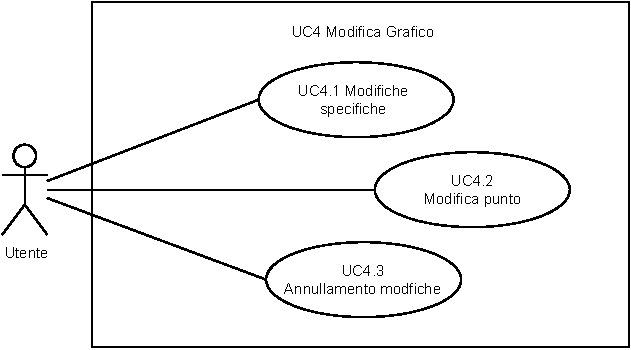
\includegraphics[width=0.5\textwidth]{componenti/casi-duso/diagrammi/UC4.pdf}
    \caption{Diagramma rappresentante UC2}
    \label{fig:UC2}
\end{figure}


\begin{itemize}
    \item \textbf{Descrizione}: L’utente vuole procedere con la fase di esplorazione
                                dati mediante la visualizzazione del dataset
                                attraverso uno dei diversi grafici proposti dall’applicativo
                                che ne costruisce uno e lo visualizza.
	
    \item \textbf{Attore primario}: Utente;
    
    \item \textbf{Precondizione}:   Nella sessione è stato importato un dataset e ogni 
                                    suo campo ha un metatag associato;

    \item \textbf{Postcondizione}:  Viene calcolato il grafico della tipologia scelta dai dati 
                                    del progetto corrente e visualizzato;

	\item \textbf{Scenario principale}:
		\begin{enumerate}
			\item L'utente seleziona l'opzione che desidera tra le tipologie di grafico:
			\begin{enumerate}
				\item Un grafico Scatterplot matrix (UC2.1.1);
				\item Un grafico Force Field (UC2.1.2);
				\item Un grafico Heat Map (UC2.1.3);
				\item Un grafico Proiezione Lineare Multiasse (UC2.4);
			\end{enumerate}
			\item HDviz visualizza il grafico ottenuto dalla costruzione dei dati;
        \end{enumerate}
	%TODO: Rimuoviamo la lista da qui? Visto che si riferisce a tutto?
    \item \textbf{Generalizzazioni:}:  L'utente seleziona il grafico desiderato:

    \begin{enumerate}
        
        \item Grafico scatterplot matrix (UC2.1).
        \item Grafico force field (UC2.2).
        \item Grafico heat map (UC2.3).
        \item Grafico proiezione lineare multiasse (UC2.4).
        
    \end{enumerate}

\end{itemize}

% TODO: Make error for each selected graph type.
\subsection{UC2.1 Selezione di Scatterplot matrix}

\begin{itemize}

    \item \textbf{Attore primario}: Utente;

    \item \textbf{Precondizione}:   Un dataset è stato correttamente importato e ad ogni campo ha associato
                                    un metatag valido;

    \item \textbf{Postcondizione}:  Viene calcolato il grafico di tipo Scatterplot matrix;
  
\end{itemize}


\subsection{UC2.2 Selezione di Force Field}

\begin{itemize}

    \item \textbf{Attore primario}: Utente;

    \item \textbf{Precondizione}:   Un dataset è stato correttamente importato e ad ogni campo ha associato
                                    un metatag valido;

    \item \textbf{Postcondizione}:  Viene calcolato il grafico di tipo Force Field;
  
\end{itemize}


\subsection{UC2.3 Selezione di Heat Map}

\begin{itemize}

    \item \textbf{Attore primario}: Utente;

    \item \textbf{Precondizione}:   Un dataset è stato correttamente importato e ad ogni campo ha associato
                                    un metatag;

    \item \textbf{Postcondizione}:  Viene calcolato il grafico di tipo Heat map dal progetto corrente
  
\end{itemize}


\subsection{UC2.4 Selezione di Proiezione lineare multiasse}

\begin{itemize}

    \item \textbf{Attore primario}: Utente;

    \item \textbf{Precondizione}:   Un dataset è stato correttamente importato e ad ogni campo ha associato
                                    un metatag;

    \item \textbf{Postcondizione}:  Viene calcolato il grafico di tipo \emph{"Proiezione lineare multiasse"} dal progetto corrente
  
\end{itemize}


